% 复叠空间：p: R -> S^1 与环路的提升
\documentclass[border=4pt]{standalone}
\usepackage{tikz}
\usetikzlibrary{arrows.meta}
\usepackage{amsmath,amssymb}
\definecolor{fillA}{rgb}{0.45,0.45,0.45}
\definecolor{fillB}{rgb}{0.72,0.72,0.72}
\begin{document}
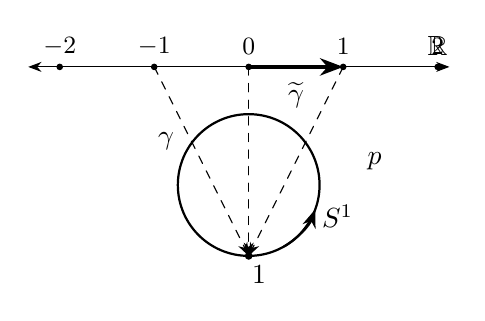
\begin{tikzpicture}[>=Stealth, line cap=round]
% 实轴 R（整数点）
\draw[<->] (1.35,4.1) -- (6.7,4.1);
\foreach \n/\x in {-2/1.75, -1/2.95, 0/4.15, 1/5.35, 2/6.55} {
  \fill (\x,4.1) circle (1.2pt);
  \node at (\x,4.36) {\small $\n$};
}
\node at (6.55,4.36) {$\mathbb R$};
% 环路 gamma 的提升（0 到 1）
\draw[very thick, ->] (4.15,4.1) -- (5.35,4.1);
\node at (4.75,3.74) {$\widetilde\gamma$};
% 复叠映射 p
\draw[dashed, ->] (2.95,4.1) -- (4.15,1.7);
\draw[dashed, ->] (4.15,4.1) -- (4.15,1.7);
\draw[dashed, ->] (5.35,4.1) -- (4.15,1.7);
\node at (5.75,2.9) {$p$};
% 基空间 S^1 与环路 gamma
\draw[thick] (5.05,2.6) arc (0:360:0.9);
\draw[thick, ->] (4.6,1.82) arc (300:340:0.9);
\node at (3.1,3.15) {$\gamma$};
\node at (5.28,2.2) {$S^1$};
% 基点 1
\fill (4.15,1.7) circle (1.4pt);
\node at (4.28,1.46) {$1$};
\end{tikzpicture}
\end{document}
